\documentclass[user_manual.tex]{subfiles}
\begin{document}
 \chapter{Primeros pasos}
 \label{x}
 Antes de poner en funcionamiento a Justina, se da a conocer el software básico con el que se trabaja y los requerimientos para  su correcto funcionamiento. También se debe saber que Justina no funciona únicamente con una computadora, trabaja con 2 actualmente; una computadora esta integrada con ubuntu 14.04.1 (esta es la version ya probada), esta es la computadora principal, la cual se encargara de todos los procesos principales de Justina y tenemos la seguna computadora (plateada) integrada con windows 7, la cual únicamente se utiliza para la comunicación: el reconocimiento por voz y la generación de voz\\
 
 \section{Software básico}
Como primer paso se debe conocer el software básico para el funcionamiento de Justina.\\

Se requiere lo siguiente:\\

-Ubuntu
\begin{itemize}
\item ROS Indigo desktop full
\item OpenNI + PrimeSense drivers
\item OpenCV 2.4.8 or 2.4.9. Compiled with OpenNi, WITHOUT OpenCL, WITHOUT Cuda, with Eigen
\item PCL 1.6
\end{itemize}

Para conocer la forma de instalar ROS, OpenNI, los drivers PrimeSense y OpenCV 2.4.9 por favor acude al apéndice B (software).\\

-Windows 7
\begin{itemize}
\item Blackboard
\item Spech recog
\item Spech generator
\end{itemize}

La comunicación entre las dos computadoras se da por medio de conexión ethernet, para esto se debe hacer una configuración punto a punto. Para conocer la configuración de la computadora por favor visite el apendice de software.

 \section{Obtención del repositorio de Github}
 Como siguiente paso se debe obtener el repositorio con el que se ha trabajado Justina.\\
 
 Todos los paquetes del software de Justina se encuentran en Github.\\
Para obtener el repositorio lo que se requiere hacer es lo siguiente: desde una terminal se debe clonar el repositorio  usado el siguiente comando:\\

\begin{minted}[
frame=lines,
framesep=1mm,
bgcolor=black,
baselinestretch=1.2
]{console}
 ~$ git clone https://github.com/RobotJustina/JUSTINA
\end{minted}
%$
 
\section{Instalación del software de Justina}
Una vez instalado ROS procedemos a instalar el software de Justina, para esto abrir una terminal y seguir las siguientes instrucciones:

\begin{enumerate}
 \item ingresamos a la carpeta JUSTINA y ejecutar JustinaSetup.sh
  \begin{center}
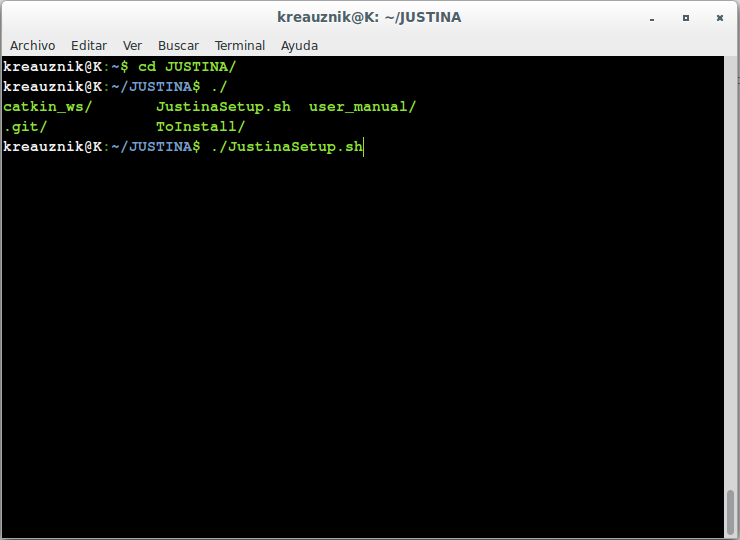
\includegraphics[width=0.73\textwidth]{Figures/PP/pp4.png}
\end{center}
 \item Confirmar cada que sea requerido. Esto nos llevara varios minutos.
 \item Una vez instalado el software, es necesario seguir las instrucciones mostradas a continuación para asociarle un nombre a los dispositivos USB conectados, y que los nombres no cambien independientemente de donde se coloquen. Cómo un enlace simbólico, el cual etiqueta al dispositivo y le asocia un nombre.

\begin{minted}[
frame=lines,
framesep=1mm,
bgcolor=black,
baselinestretch=1.2
]{console}
 ~$ sudo cp 80-justinaRobot.rules /etc/udev/rules.d/
\end{minted}
%$ 
 
 \item Una vez termines de ejecutar el comando, es necesario ejecutar el siguiente: 
 
\begin{minted}[
frame=lines,
framesep=1mm,
bgcolor=black,
baselinestretch=1.2
]{console}
 ~$ sudo udevadm control --reload-rules && sudo service udev restart 
 && sudo udevadm trigger
\end{minted}
%$

 
\end{enumerate}
Listo, ya está instalado el software de Justina.

\section{Cómo compilar los paquetes de Justina}
Para compilar los paquetes de Justina se debe acceder al siguiente directorio " JUSTINA/catkin\_ws", en este directorio se debe ejecutar el siguiente comando: 

\begin{minted}[
frame=lines,
framesep=1mm,
bgcolor=black,
baselinestretch=1.2
]{console}
 ~$ catkin_make
\end{minted}
%$

Una vez compilados todos los paquetes, es necesario ejecutar el siguiente comando dentro del mismo directorio:

\begin{minted}[
frame=lines,
framesep=1mm,
bgcolor=black,
baselinestretch=1.2
]{console}
 ~$ source devel/setup.bash
\end{minted}
%$

 \begin{center}
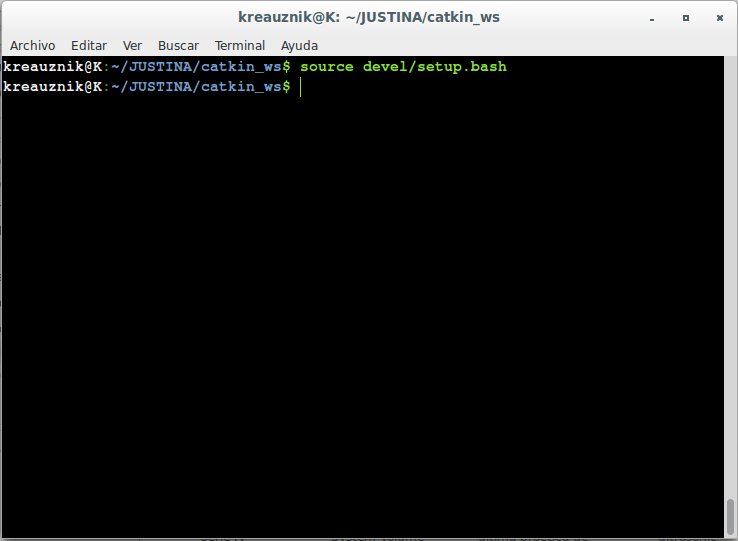
\includegraphics[width=0.73\textwidth]{Figures/PP/pp5.png}
\end{center}

Por conveniencia es necesario agregar esto a tu .bashrc:\\

\begin{minted}[
frame=lines,
framesep=1mm,
bgcolor=black,
baselinestretch=1.2
]{console}
 ~$ echo "source ~/catkin_ws/devel/setup.bash" >> ~/.bashrc
\end{minted}
%$

Además se debe adherir el workspace a:\\

\begin{minted}[
frame=lines,
framesep=1mm,
bgcolor=black,
baselinestretch=1.2
]{console}
 ~$ echo "export ROS_PACKAGE_PATH=$ROS_PACKAGE_PATH:~/catkin_ws" >> ~/.bashrc
\end{minted}
%$

Listo, ahora el software de Justina está instalado y los paquetes compilados y listos para usarse.

\end{document}
